%\clearpage
%\subsection{Signal Uncertainties}
\label{subsec:sig_uncer}


\subsection{PDF and Scale uncertainties}
\label{subsec:sig_uncer_scales_PDF}

Similar to the treatment of backgrounds, additional systematic uncertainties arise for signals due to modeling differences among various signal MC generators. 
These uncertainties include PDF uncertainties and QCD scale uncertainties for signal samples generated using Next-to-Leading Order (NLO) QCD. 
These uncertainties, which affect signal acceptance, are analyzed using truth weight information stored in the current analysis framework.

For the scale uncertainty, we adopt the envelope method employing the usual variations, akin to the approach utilized for background samples, as detailed in Section \ref{subsec:scale_pdf_unc}. Examples of these uncertainties are illustrated in Figures \ref{fig:PDFUnc1Lep_sig} through \ref{fig:ScaleUnc1Lep_sig}.

\begin{figure}[ht]
    \centering
    \begin{subfigure}[b]{0.3\textwidth}
        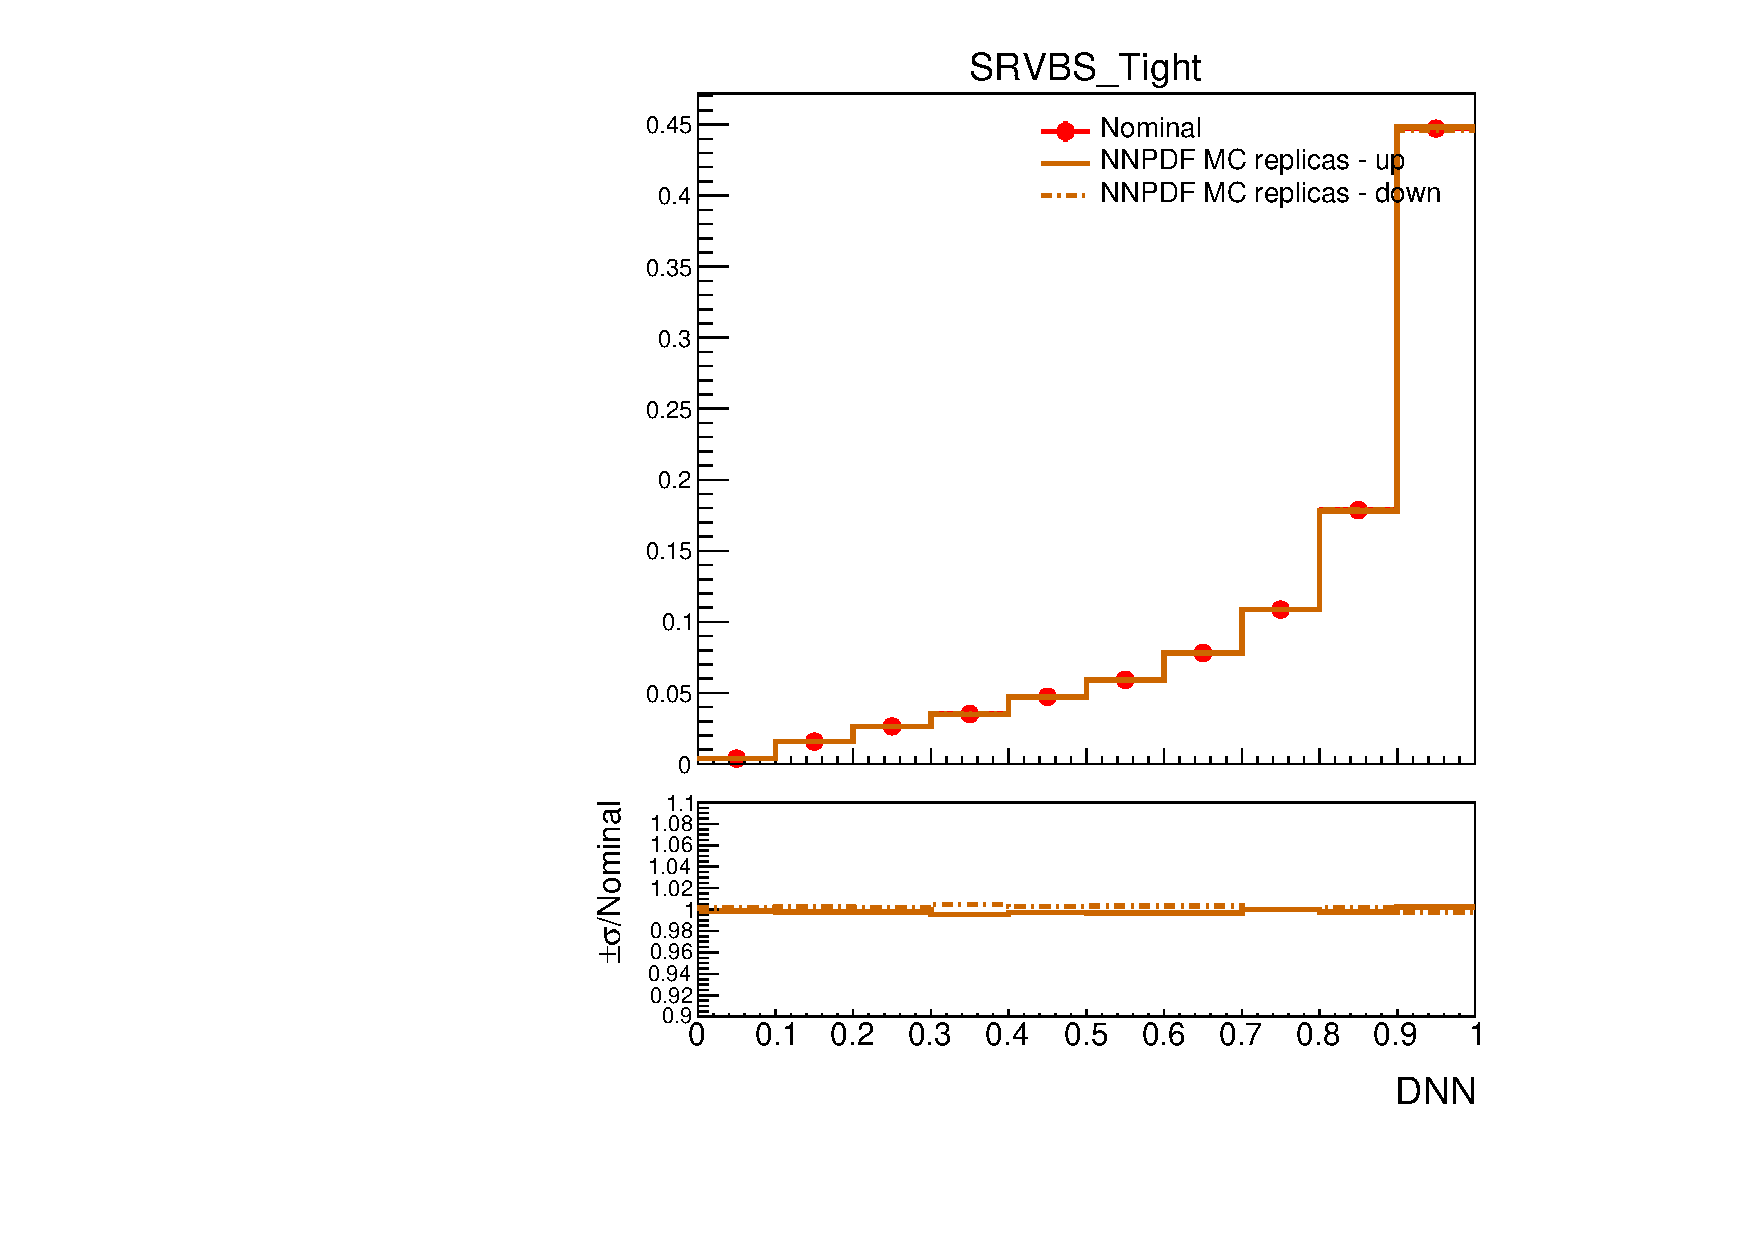
\includegraphics[width=\textwidth]{figures/1lep/PDFUnc/NNPDF_DNN/EW6lvqq_0ptag2pjet_0ptv_SRVBS_Tight_DNN_SysTheoryPDF_NNPDF_VBS__1up_Norm.pdf}
        \caption{Resolved SR}
    \end{subfigure}
    \begin{subfigure}[b]{0.3\textwidth}
        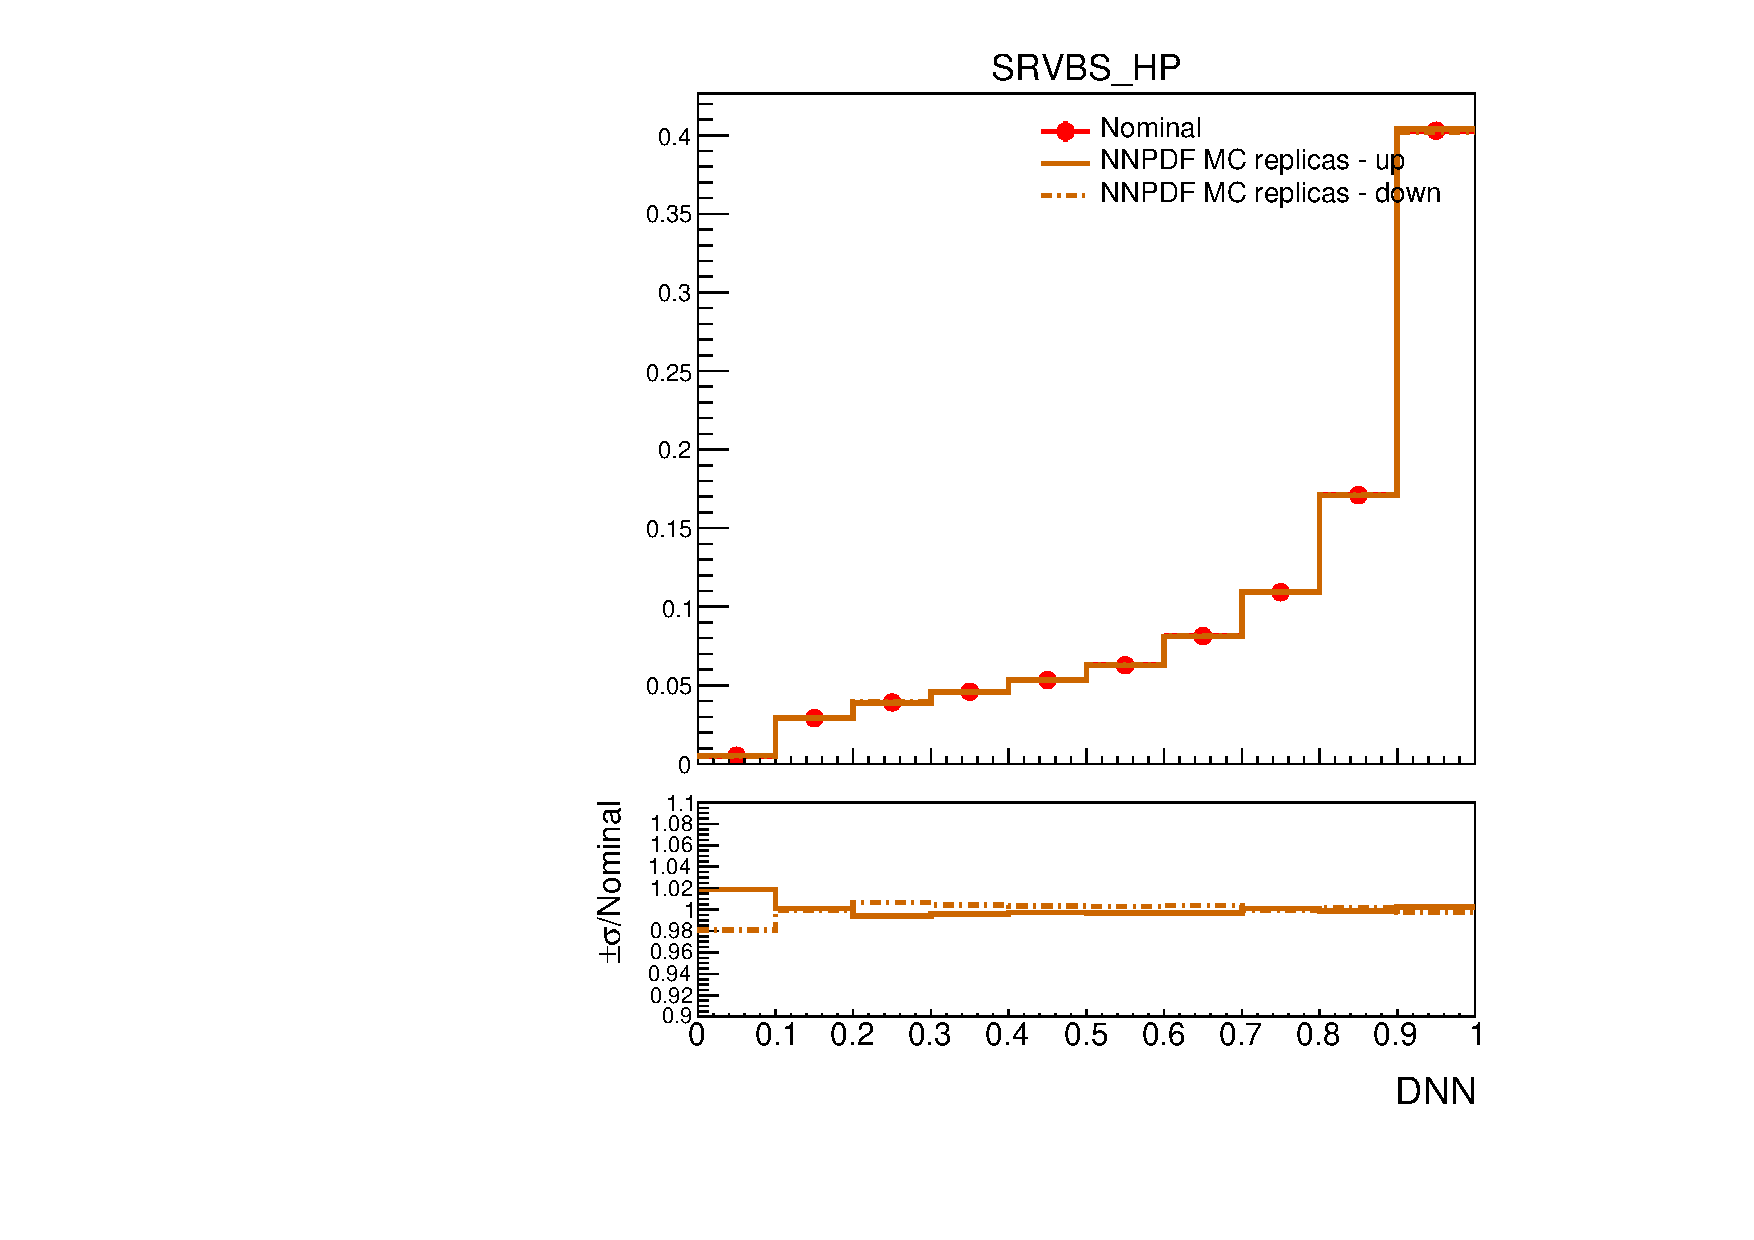
\includegraphics[width=\textwidth]{figures/1lep/PDFUnc/NNPDF_DNN/EW6lvqq_0ptag1pfat0pjet_0ptv_SRVBS_HP_DNN_SysTheoryPDF_NNPDF_VBS__1up_Norm.pdf}
        \caption{Merged HP SR}
    \end{subfigure}
    \begin{subfigure}[b]{0.3\textwidth}
        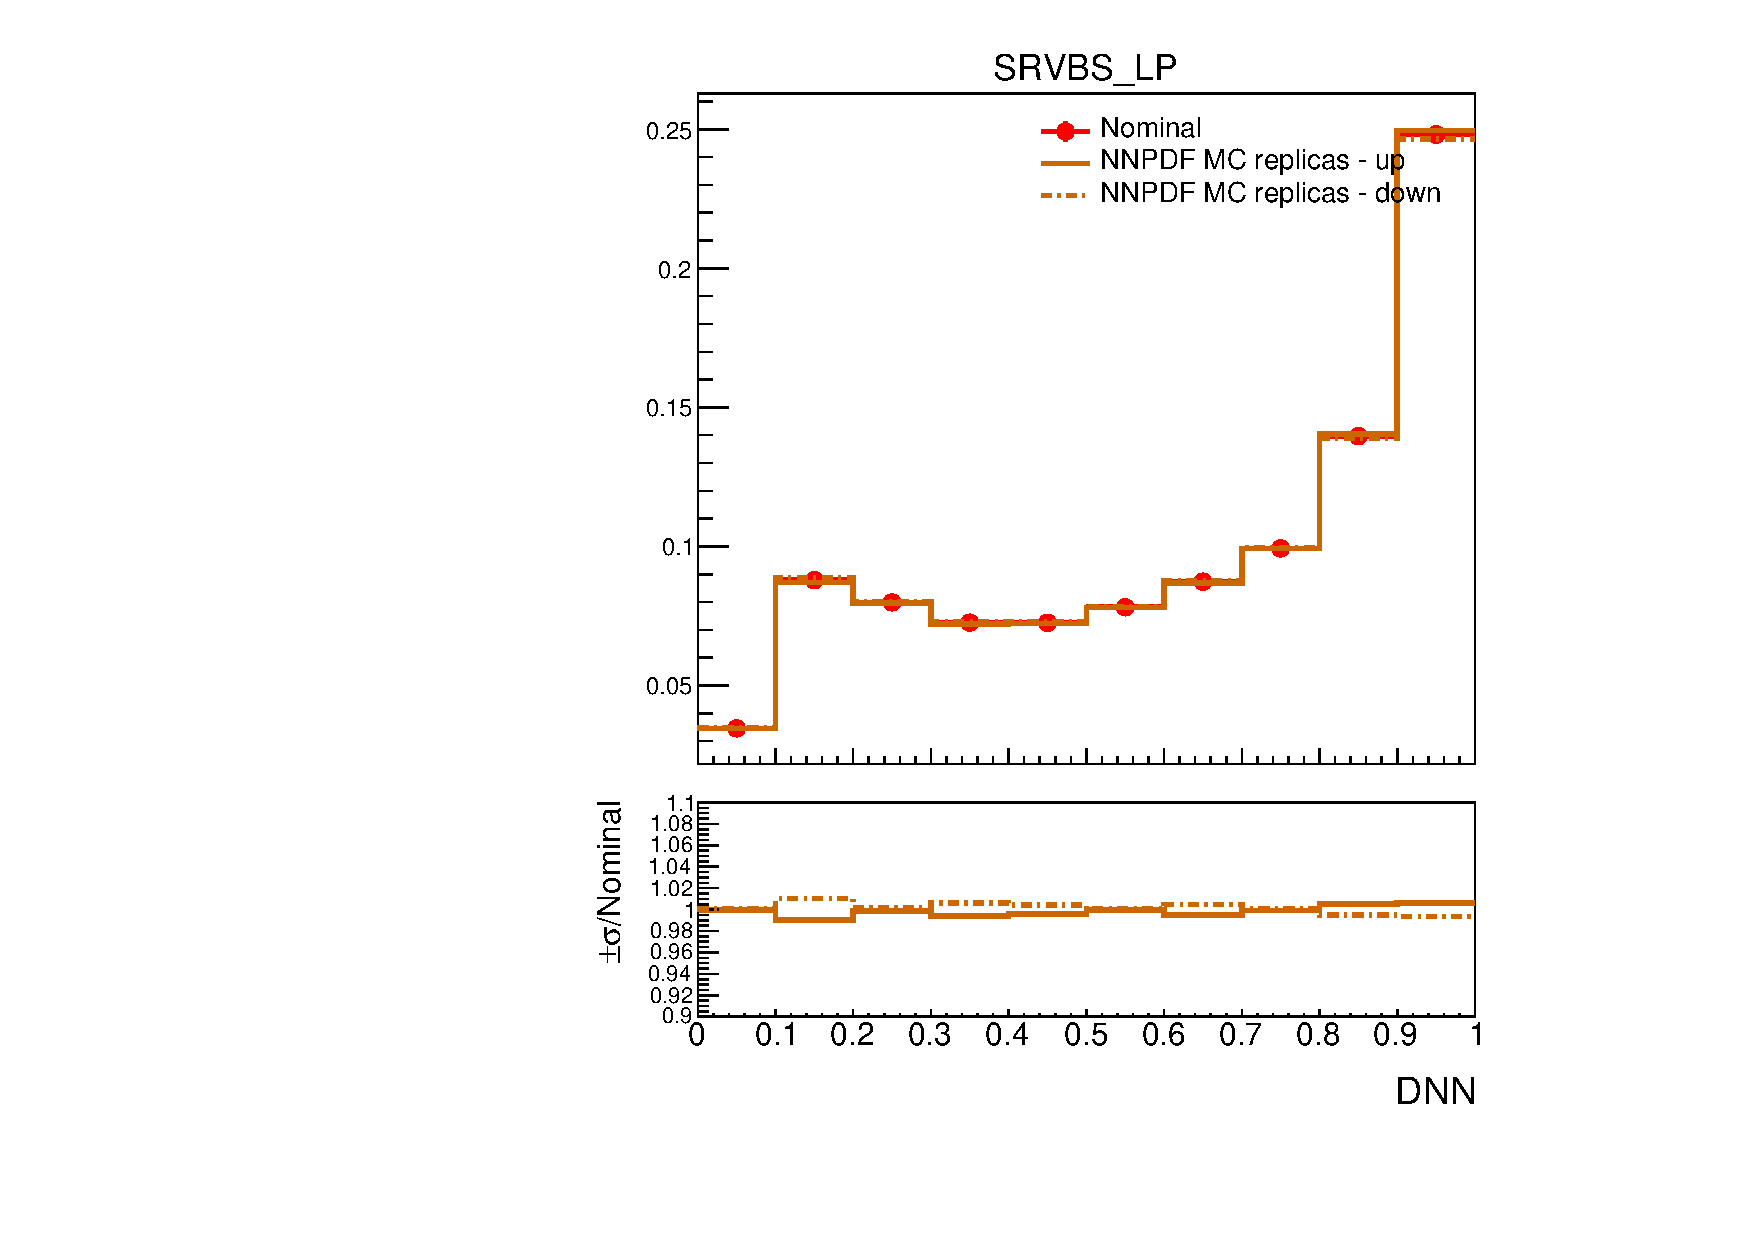
\includegraphics[width=\textwidth]{figures/1lep/PDFUnc/NNPDF_DNN/EW6lvqq_0ptag1pfat0pjet_0ptv_SRVBS_LP_DNN_SysTheoryPDF_NNPDF_VBS__1up_Norm.pdf}
        \caption{Merged LP SR}
    \end{subfigure}
    \caption{PDF uncertainties of the signal MC sample in the 1-lepton channel. Histograms are normalized.}
    \label{fig:PDFUnc1Lep_sig}
\end{figure}


\begin{figure}[ht]
    \centering
    \begin{subfigure}[b]{0.3\textwidth}
        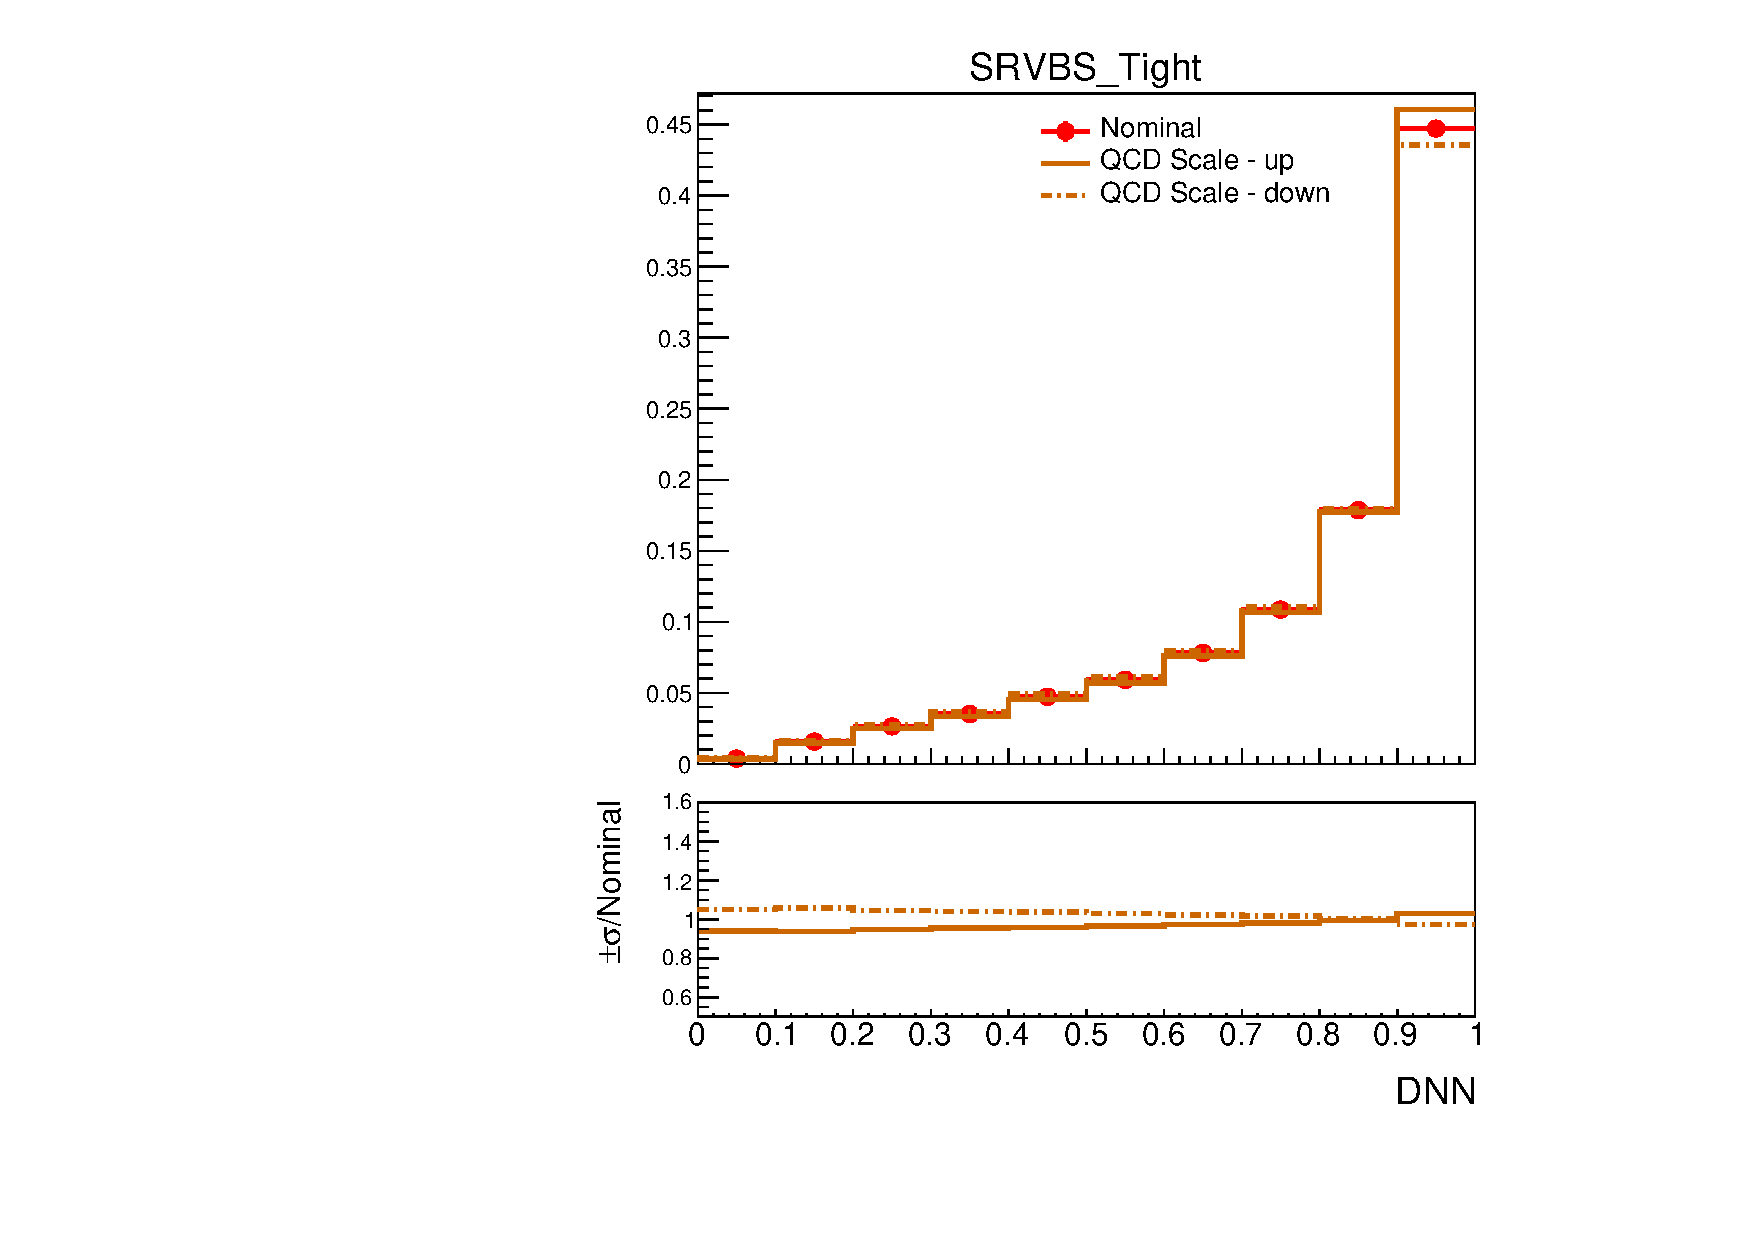
\includegraphics[width=\textwidth]{figures/1lep/PDFUnc/QCDScale_DNN/EW6lvqq_0ptag2pjet_0ptv_SRVBS_Tight_DNN_SysTheoryQCD_VBS__1up_Norm.pdf}
        \caption{Resolved SR}
    \end{subfigure}
    \begin{subfigure}[b]{0.3\textwidth}
        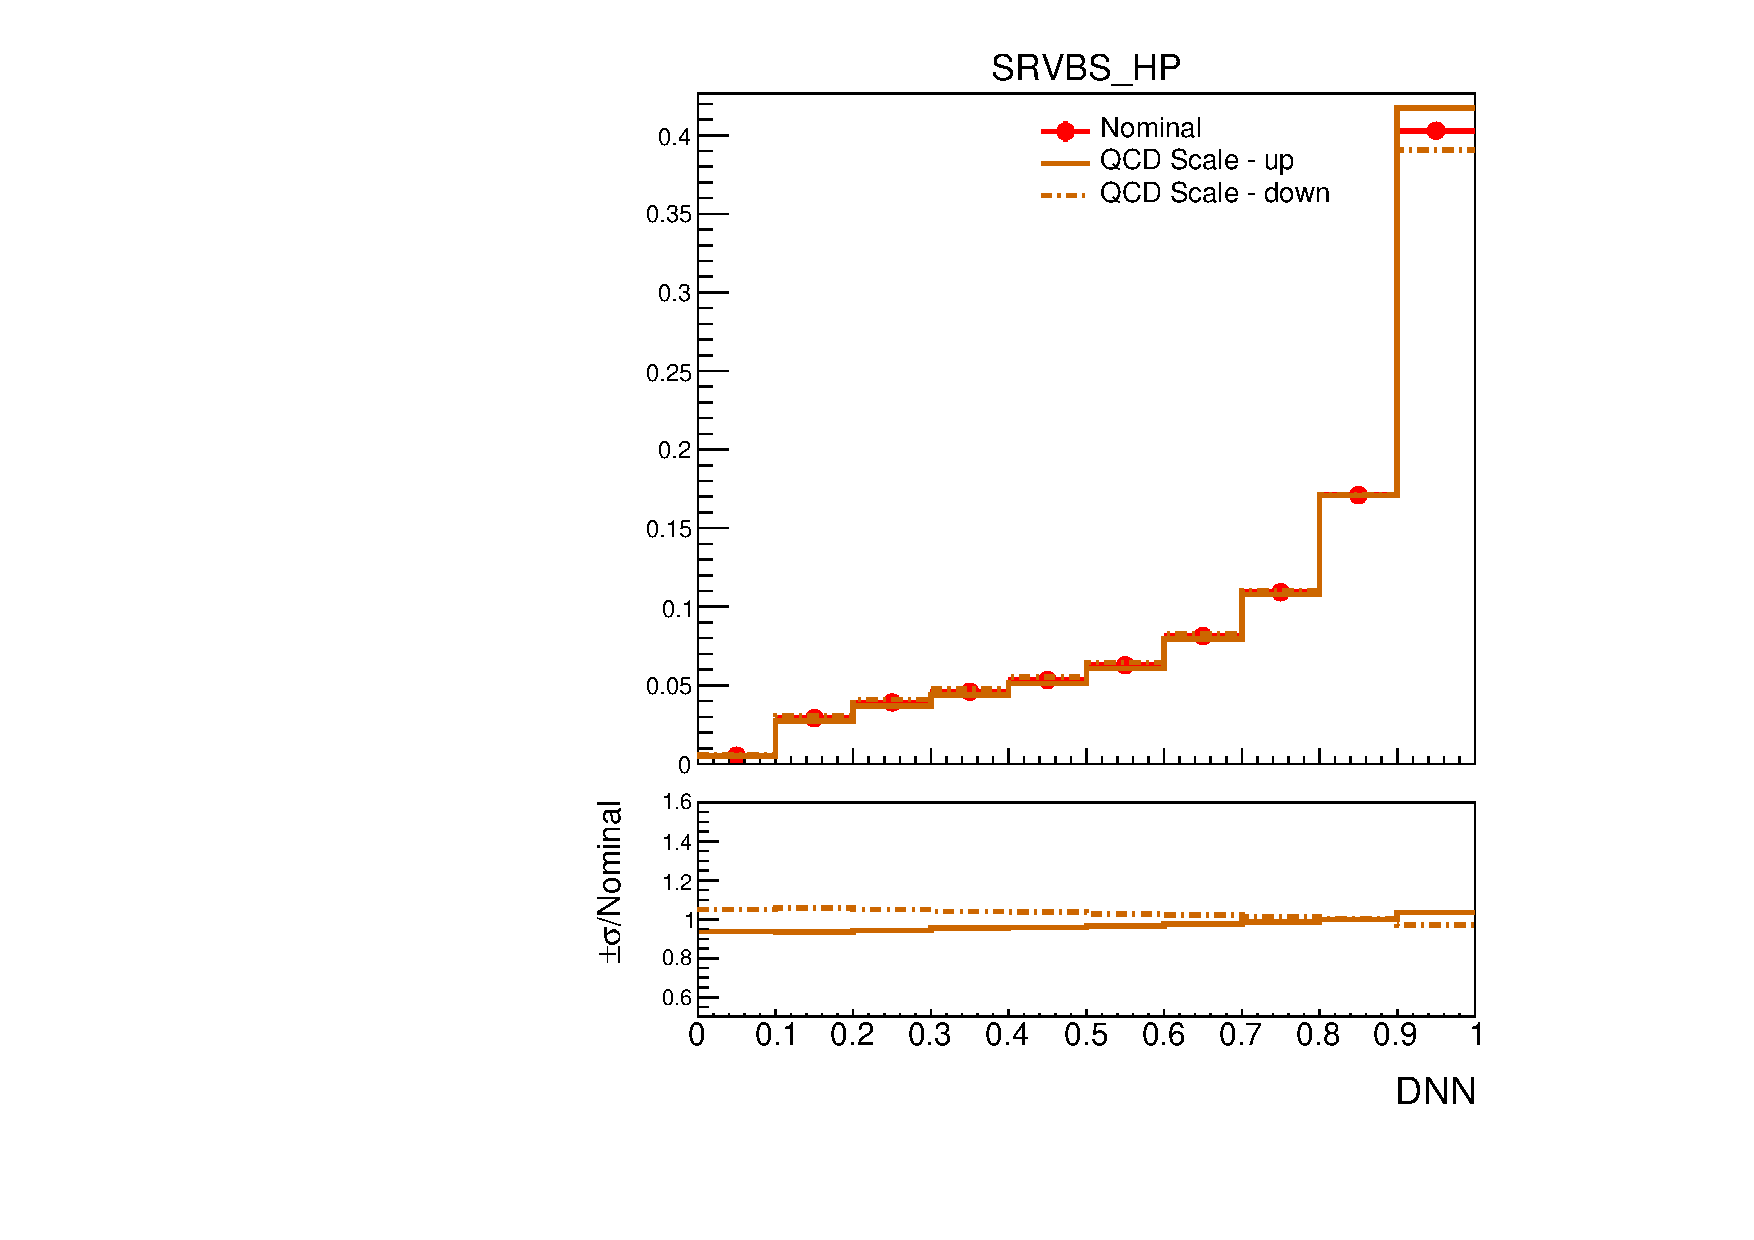
\includegraphics[width=\textwidth]{figures/1lep/PDFUnc/QCDScale_DNN/EW6lvqq_0ptag1pfat0pjet_0ptv_SRVBS_HP_DNN_SysTheoryQCD_VBS__1up_Norm.pdf}
        \caption{Merged HP SR}
    \end{subfigure}
    \begin{subfigure}[b]{0.3\textwidth}
        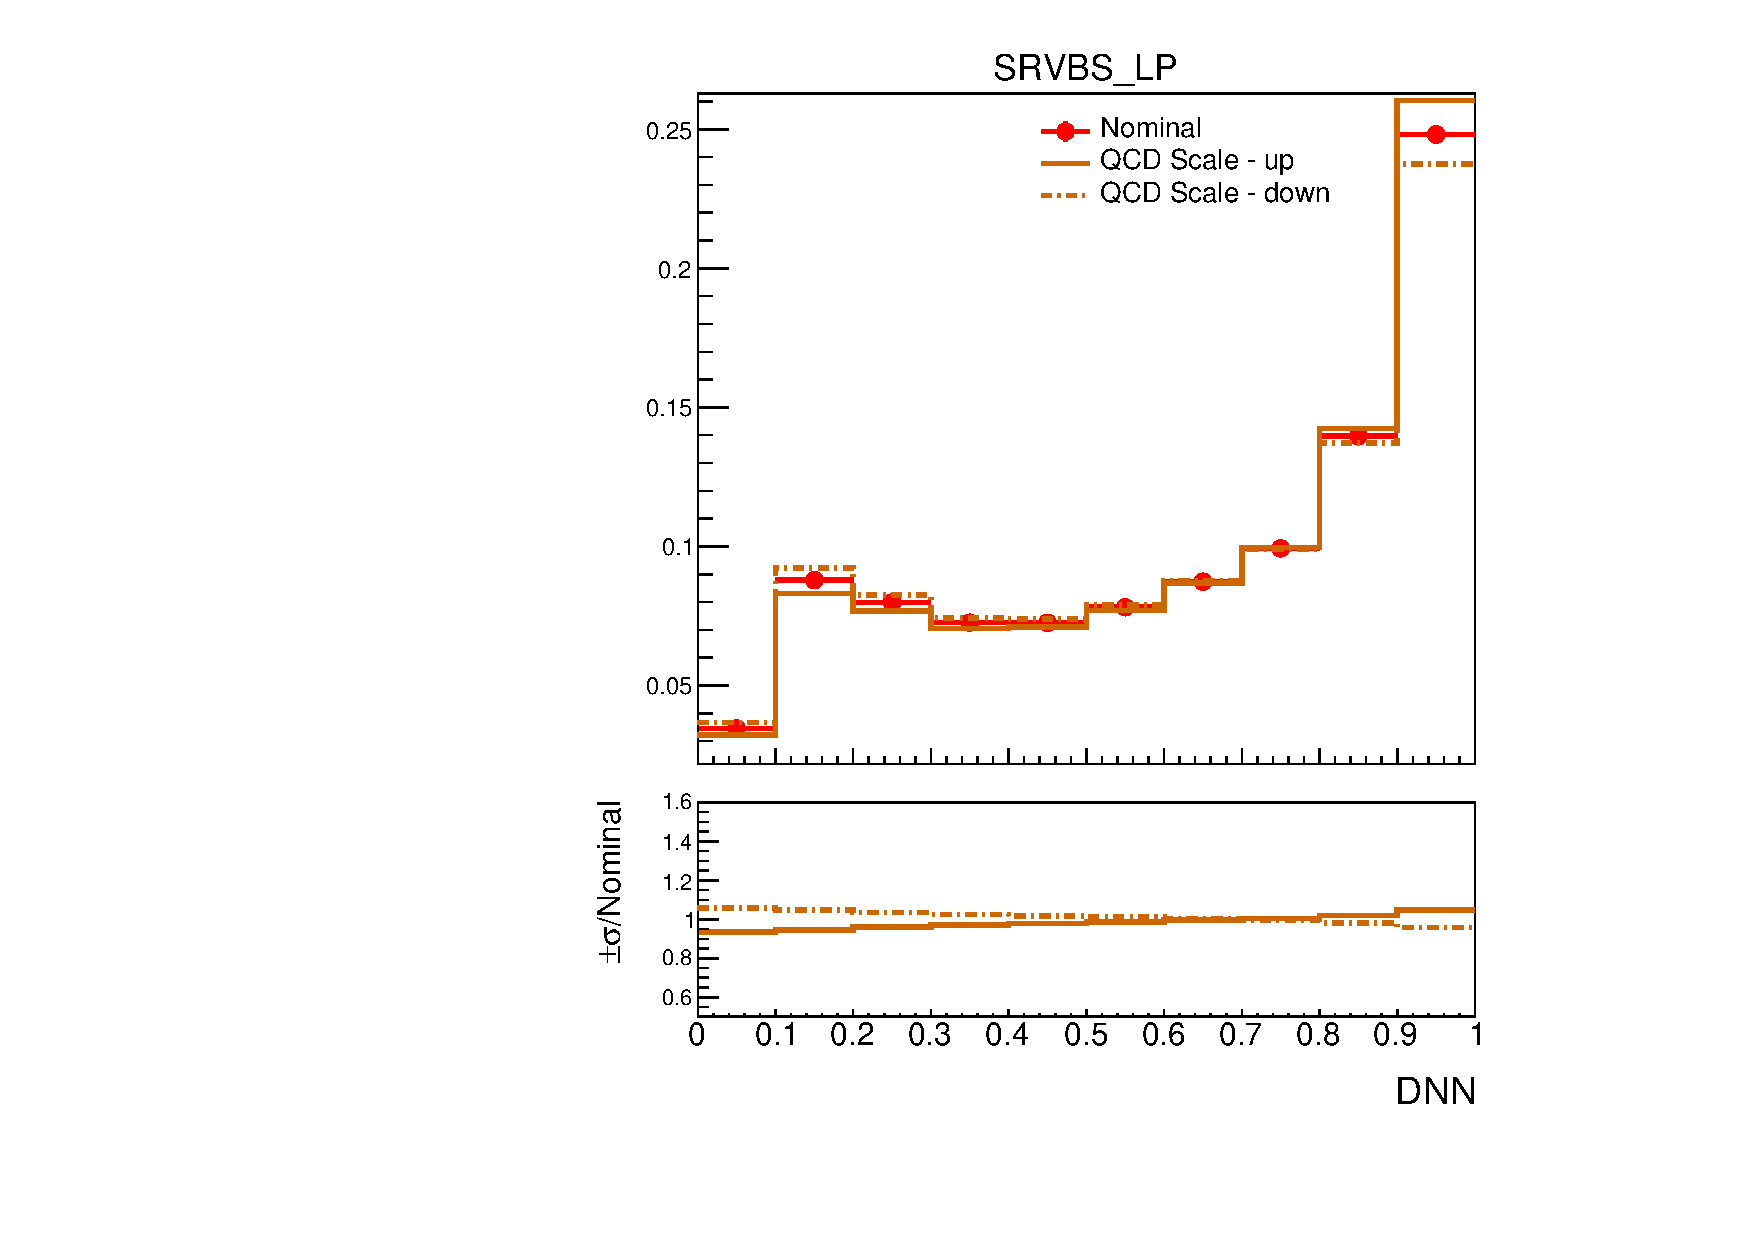
\includegraphics[width=\textwidth]{figures/1lep/PDFUnc/QCDScale_DNN/EW6lvqq_0ptag1pfat0pjet_0ptv_SRVBS_LP_DNN_SysTheoryQCD_VBS__1up_Norm.pdf}
        \caption{Merged LP SR}
    \end{subfigure}
    \caption{QCD scale uncertainties of the signal MC sample in the 1-lepton channel. Histograms are normalized.}
    \label{fig:ScaleUnc1Lep_sig}
\end{figure}

\clearpage
\subsection{EWK-QCD interference and Shower uncertainty}
\label{subsec:sig_uncer_interf}

Due to time constraints and the extensive scope of this study, certain aspects could not be comprehensively addressed, including the potential effects of Electroweak-Quantum Chromodynamics (EWK-QCD) interference and the impact of parton showering on the signal MC samples. 
Notably, the EWK and QCD vector boson plus jets (VV+jj) samples were generated separately, implying that no interference contributions were considered in the analysis. While these factors are acknowledged for their potential minor impact on the results, a detailed investigation was beyond the scope of this thesis. Alternative MC samples necessary for assessing these uncertainties were not available when my DNN study concluded. Future studies could explore these aspects to enhance the understanding of the systematics involved.

